\subsubsection{Reconfiguration with compensation in case of angular velocity sensor fault}

A reconfiguration scheme using anomaly detection in angular velocity sensors has been implemented in the simulation. The detection checks the magnitude of the angular velocity gradient, and if it's above the threshold, the supervisor shuts down the corresponding wheel in a controlled fashion and distributes the torque demand to the remaining wheels. This is necessary, since the reaction wheel control scheme relies on angular velocity measurements. 

It is imperative to compensate for the torque output of the faulty wheel for the satellite dynamics not to be affected by the fault. If the control voltage of the wheel is instantaneously turned off to zero at the moment the fault is detected, the torque output of the wheel can be quite large due to the fast deceleration, making compensation more problematic. Instead the control voltage should be decreased more slowly to reduce the torque output. The torque output of the faulty wheel can not be derived from angular velocity measurements in the presence of an angular velocity sensor fault. In order to be able to compensate for the deceleration torque, using the assumption that the only fault is in the sensor, wheel deceleration can be simulated based on the model, and compensation can be done for the simulated torque output of the wheel.

The shut down happens as follows: when the sensor fault is detected, the system registers the momentary control voltage at the input of the faulty wheel, and starts slowly decreasing the voltage to zero. In parallel, a simulation starts for wheel deceleration with the angular velocity initial value being the last non-faulty value. The voltage input of the simulation is always the same as for the real system. As the fault occurs, the reaction wheel torque distribution is changed to omit the faulty wheel. The simulated torque output of the wheel faulty wheel is fed to the reaction wheel torque distributor for compensation.

\begin{figure}
	\centering
	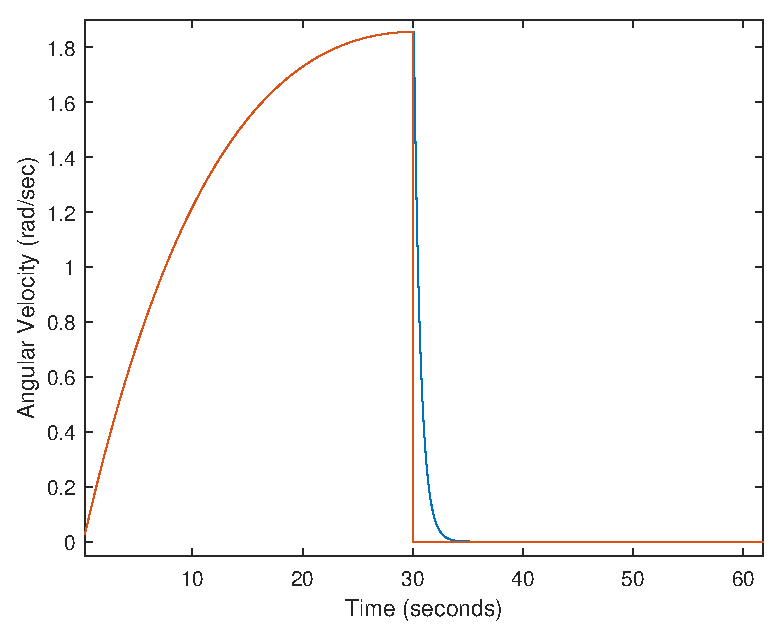
\includegraphics[width=120mm]{figures/omegaSensorfault_omega}
	\caption{$\omega_{M,i}$ sensor signal and actual value with fault occuring at 30 seconds}
\end{figure} 

\begin{figure}
	\centering
	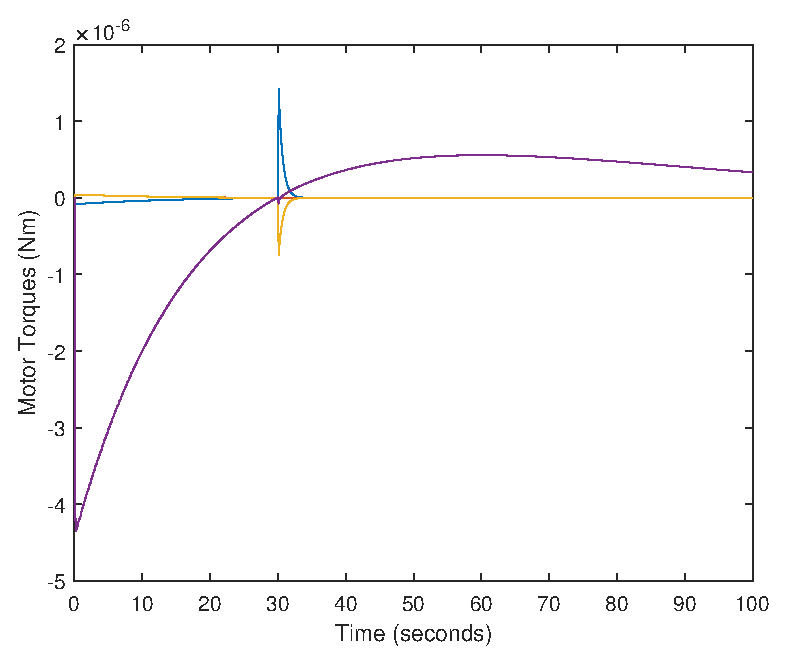
\includegraphics[width=120mm]{figures/omegaSensorfault_Nmotor}
	\caption{$N_M$ with $\omega$ sensor fault occuring at 20 seconds}
\end{figure} 

\begin{figure}
	\centering
	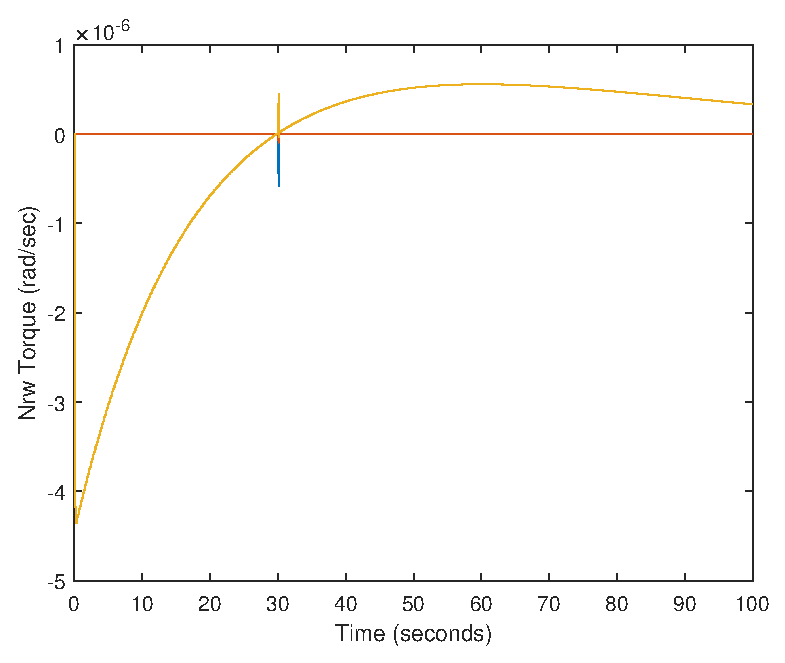
\includegraphics[width=120mm]{figures/omegaSensorfault_Nrw}
	\caption{$N_{rw}$ with $\omega$ sensor fault occuring at 20 seconds}
\end{figure} 
